\section{Supplemental Results}\label{sup}
%\subsection{Binomial Adjustment: Examples of Bias}\label{sup.bin} % TODO
\begin{figure}[h]
  \centerline{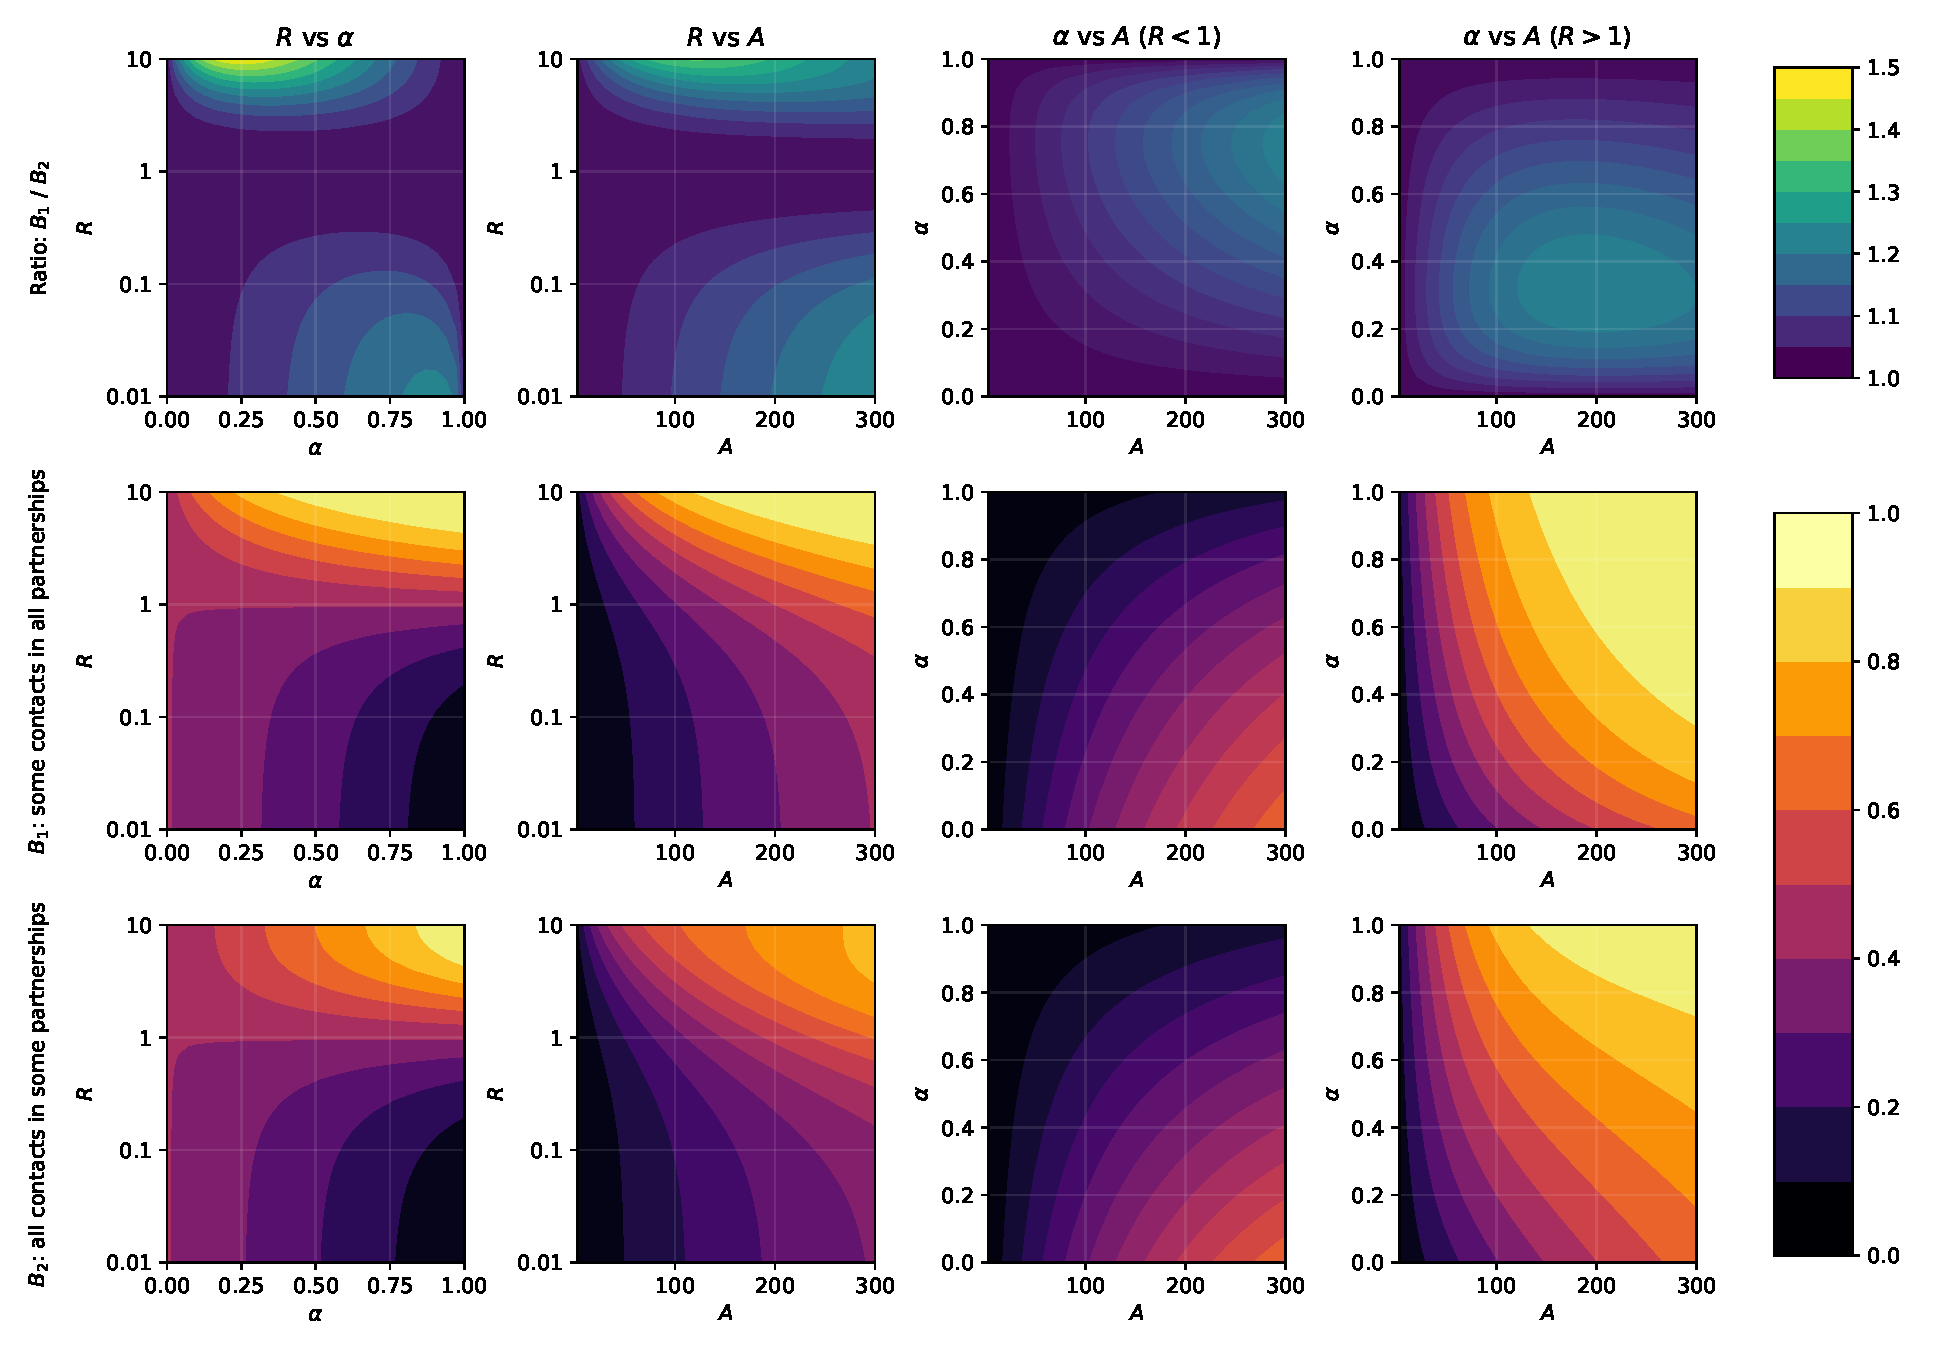
\includegraphics[width=\widefig]{B.mod.vs}}
  \caption{Per-partnership probability of transmission $B$,
    in the presence of a transmission modifier $R$, calculated assuming either:
    $B_1$: $\alpha$ proportion of contacts in all partnerships modified; or
    $B_2$: all contacts in $\alpha$ proportion of partnerships modified.
    We observe $B_1 \ge B_2$.}
  \label{fig:B.mod.sens}
  \floatfoot
  $\beta = 0.34\%$ throughout \cite{Boily2009}.
  For $R$ vs $\alpha$, $A = 152$;
  for $R$ vs $A$, $\alpha = 0.5$;
  for $\alpha$ vs $A$, $(R<1) = 0.1$, $(R>1) = 5$.
  For $0.1 < R < 3$, the ratio $B_1 / B_2 \approx 1$.
  When $R < 1$, then $B_1 / B_2$ is maximized with $A \rightarrow \infty$ and $0.5 < \alpha < 1$.
  When $R > 1$, then $B_1 / B_2$ is maximized with $1 < A < \infty$ and $0 < \alpha < 0.5$.
\end{figure}